\documentclass[reprint,amsmath,amssymb,aps,prb]{revtex4-2}

\usepackage{graphicx}% Include figure files
\usepackage{dcolumn}% Align table columns on decimal point
\usepackage{bm}% bold math
\usepackage{hyperref}% add hypertext capabilities
\usepackage{xcolor}
\usepackage{braket}
\usepackage[english]{babel}

%% Philipps stuff %%
\usepackage[font={small}]{caption}
\usepackage{subcaption}
\captionsetup[subfigure]{list=true, font=small, labelfont=bf, 
	labelformat=brace, position=top}
\usepackage{amsmath}
\def\arraystretch{1.5}
\usepackage{float}
\usepackage{lipsum}


%% Code stuff %%
\usepackage{listings} % insert code fragments

\definecolor{codegreen}{rgb}{0,0.6,0}
\definecolor{codegray}{rgb}{0.5,0.5,0.5}
\definecolor{codepurple}{rgb}{0.58,0,0.82}
\definecolor{backcolour}{rgb}{0.95,0.95,0.92}

\lstdefinestyle{mystyle}{
    backgroundcolor=\color{backcolour},   
    commentstyle=\color{codegreen},
    keywordstyle=\color{magenta},
    numberstyle=\tiny\color{codegray},
    stringstyle=\color{codepurple},
    basicstyle=\ttfamily\footnotesize,
    breakatwhitespace=false,         
    breaklines=true,                 
    captionpos=b,                    
    keepspaces=true,                 
    numbers=left,                    
    numbersep=5pt,                  
    showspaces=false,                
    showstringspaces=false,
    showtabs=false,                  
    tabsize=2
}

\lstset{style=mystyle}

\begin{document}

%\title{Project title}

\author{Your Name}

\date{\today}% It is always \today, today,
             %  but any date may be explicitly specified

\begin{abstract}
A paper usually includes an abstract, a concise summary of the work covered at length in the main body of the paper. Please also write a short abstract of your project.
\end{abstract}


\maketitle




\section{Guidelines}



Please write a short paper about your project. There are no strict length limits, but please write \textbf{at least two pages in the layout of this template} (including figures, excluding references and code listings). Please structure your paper in a scientific way, and include your references and your code. There are \LaTeX packages you can use to preserve the indentation of your code, e.g. the \texttt{listings} package which is demonstrated in the Appendix~\ref{app:codes}.

This sample document makes use of of REV\TeX~4.2, therefore you will need to install it to be able to compile this document yourself. Further information can be found in the REV\TeX~4.2
documentation included in the distribution or available at
\url{http://journals.aps.org/revtex/}.



\subsection{Example citations}
By default, citations are numerical\cite{epr}, some more citations~\cite{feyn54,Bire82,Berman1983,witten2001,Davies1998}. 

\subsection{Exampe figure}
Including and referring to figures is as usual, see for instance Fig.~\ref{fig:example}
\begin{figure}
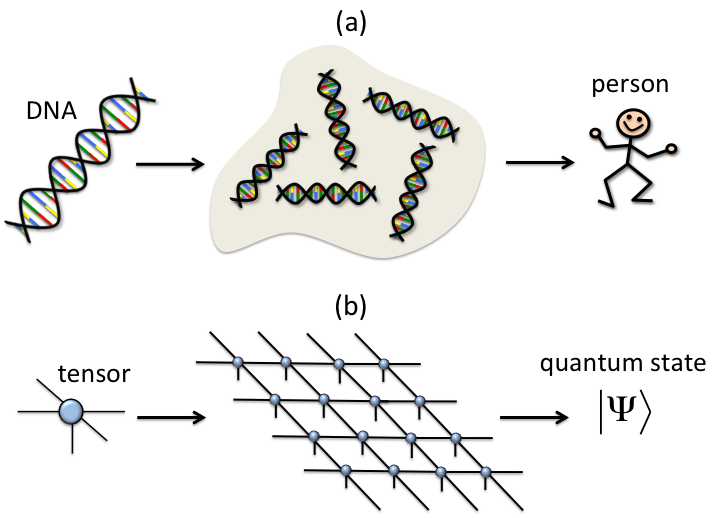
\includegraphics[width=0.99\linewidth]{cartoon.png}
\caption{Example of a figure~\cite{Orus2013}.}
\label{fig:example}
\end{figure}

\bibliography{bibsamp}% Produces the bibliography via BibTeX.


\appendix


\begin{widetext}
\section{Code listing} \label{app:codes}
Please copy your code in the appendix.
\begin{lstlisting}[language=Python]
"""

Module to generate the Hamiltonian of the transverse field Ising model.

H = -J sum_i sigma^x_i sigma^x_{i+1} - g sum_i sigma^z i.

Used in the solution of exercise 5.1

"""

import numpy as np
import scipy
from scipy import sparse
import scipy.sparse.linalg
import matplotlib.pyplot as plt

Id = sparse.csr_matrix(np.eye(2))
Sx = sparse.csr_matrix([[0., 1.], [1., 0.]])
Sz = sparse.csr_matrix([[1., 0.], [0., -1.]])
Splus = sparse.csr_matrix([[0., 1.], [0., 0.]])
Sminus = sparse.csr_matrix([[0., 0.], [1., 0.]])


def singesite_to_full(op, i, L):
    op_list = [Id]*L  # = [Id, Id, Id ...] with L entries
    op_list[i] = op
    full = op_list[0]
    for op_i in op_list[1:]:
        full = sparse.kron(full, op_i, format="csr")
    return full


def gen_sx_list(L):
    return [singesite_to_full(Sx, i, L) for i in range(L)]


def gen_sz_list(L):
    return [singesite_to_full(Sz, i, L) for i in range(L)]


def gen_hamiltonian_periodic(sx_list, sz_list, g, J=1.):
    """ assumes periodic boundery conditions """
    L = len(sx_list)
    H = sparse.csr_matrix((2**L, 2**L))
    for j in range(L):
        H = H - J *( sx_list[j] * sx_list[(j+1)%L])
        H = H - g * sz_list[j]
    return H
\end{lstlisting}
\end{widetext}

\title{Machine Learning of Many Body Localization}

\author{Philipp Krüger}

\date{\today}% It is always \today, today,
             %  but any date may be explicitly specified

\begin{abstract}
The goal of this study was to find the quantum phase transition at intermediate local disorder strengths on a Heisenberg chain. Exact diagonalization was used to find the reduced density matrices for a different number of consecutive spins for the lowest energy eigenstate of the Heisenberg Model with an additional random field in z-direction at low and high disorder strengths. The resulting dataset representing extended and localized phases was used to train a neural network. Afterwards, the trained network was applied on intermediate disorder strengths to deduct the critical disorder strength for a phase transition. This phase transition was for all system sizes predicted to be around $W_c = 1.5 J$ for the system sizes $L\in\{9, 10, 11, 12\}$ and block sizes $n\in\left[1,7\right]$. Low block sizes suffered from a low accuracy in the machine learning model, whereas for higher block sizes the $W_c$ values approached $W_c=J$.  %todo system size? Block size? ML model performance and Wc dependency
\end{abstract}

\maketitle

\section{Introduction}

The physical model and the concept of exact diagonalization is presented first. As we use reduced density matrices as features for the neural network, we explain briefly their computation and meaning.
%Review Literature on task. How other people find $W_c$?
%Why is the topic interesting? => Finding Wc?
\subsection{Physical model}

\subsubsection{Hamiltonian of the Heisenberg model}

The Hamiltonian of the Heisenberg model is shown in equation \ref{hamiltonian}. In the course of further analysis, we choose $J=1$ and sample $h$ from a uniform distribution such that $h_i \in \left[-W, W\right]$.

\begin{equation}
	H=\underbrace{J\sum_i \vec{S}_i\cdot\vec{S}_{i+1}}_{\text{Exchange Energy}}-\underbrace{\sum_ih_iS_i^z}_{\text{Random Field}}\label{hamiltonian}
\end{equation}

%todo: nice picture with spins and all?

\subsubsection{Expectations for the ground state}
%todo:
\url{https://journals.aps.org/prb/abstract/10.1103/PhysRevB.91.081103}


The expectation for the ground state is dependent on the ratio of the coupling and the local random field. 

For $\frac{W}{J} \ll 1$, we expect an delocalized, extended phase, since the exchange energy dominates over the small external field. Therefore, the system can relax to thermal equilibrium serving as its own heat bath in the limit of large system size $L\rightarrow\infty$.
Here, the reduced density operator of a finite subsystem converges to the equilibrium thermal distribution
for $L\rightarrow\infty$.\cite{Pal2010}

For $\frac{W}{J} \gg 1$, we can expect a localized phase, since the $h_i$ factors dominate over the exchange energy. The resulting states are expected to be product states of spins "up" or "down", as the external field points in z-direction. Also an infinite system cannot equilibrate itself. The local configurations are set by the initial conditions at all times and are adiabatically connected to the trivial state.\cite{Pal2010}

%\begin{figure}
%	\centering
%	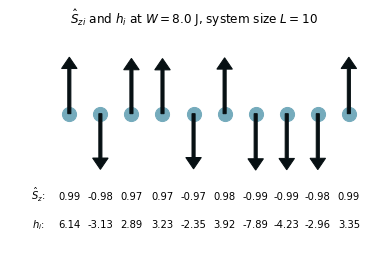
\includegraphics[width=1\linewidth]{figures/heisenberg_chain}
%	\caption{Visualization of the random disorder strength efftect on a ground state.}
%	\label{fig:heisenberg_chain}
%\end{figure}

\subsection{Exact diagonalization}

Exact diagonalization (ED) is a numerical technique we can use to solve the time independent Schrödinger Equation $H\ket{\psi}=E\ket{\psi}$ for the eigenvalues $E$ and eigenvectors $\ket{\psi}$. This only works of the Hamiltonian $H$ represents a discrete and finite system. Most quantum many-particle problems lead to a sparse matrix representation of the Hamiltonian, where only a very small fraction of the matrix
elements is non-zero.\cite{Weisse2008} An efficient method to find ground states is the Lanczos algorithm.\cite{Lanczos1950} At first, the algorithm was numerically unstable. This issue was overcome in 1970 by Ojalvo and Newman.\cite{Ojalvo1970} In this study, we rely on the Lanczos algorithm for the eigensolver.

\subsection{Reduced Density Matrix}

The usefulness of reduced density matrices has already been shown by White in 1992 with ground states of Heisenberg chains \cite{White1992}. In our case we use areal density matrices as features for the neural network to predict the critical disorder strength of a phase change from delocalized to localized. The reduced density matrix is defined in equation \ref{red_density}. Physically, the reduced density matrix $\rho_A$, provides correct measurement statistics for subsystem A.

\begin{eqnarray}
\rho_{AB}&=&\ket{\psi_A}\bra{\psi_A}\otimes\ket{\psi_B}\bra{\psi_B}\\
\rho_A&=&\text{Tr}_B(\rho_{AB})=\ket{\psi_A}\bra{\psi_A}\text{Tr}\left(\ket{\psi_B}\bra{\psi_B}\right)\label{red_density}
\end{eqnarray}%\url{http://www.thphys.nuim.ie/staff/jvala/Lecture_9.pdf}

The reduced density matrix was also used by Zhang in 2019 to learn the localization transition in disordered quantum Ising spin chains. Here, the motivation was to reduce the dimension and filter out redundant information. However, it proved to be inferior in comparison to the full density matrix in the analysis. \cite{Zhang2019} However, due to RAM limitations, we will rely on reduced density matrices.


\subsection{Artificial Neural Networks}

Rosenblatt published in 1958 his concept of the probabilistic model for information storage and organization in the brain, which greatly inspired others to use those models for computation.\cite{Rosenblatt1958} Over the course of years, they have evolved to a tool that can be used for a variety of applications including computer vision, speech recognition, medical diagnosis, playing games or even artistic painting.\cite{Gatys2015}

The reduced density matrices are essentially complex 2D arrays with length $2^n\times2^n$. As we want to classify for an arbitrary $W$ whether we have a localized or delocalized phase, it is convenient to use a machine learning classifier. The density matrices can then be thought of as a complex and real image that can be fed into it analogously to classical image classification.


\section{Computational Methods}

The strategy for implementation was as follows:

\begin{enumerate}
	\item Generate Hamiltonian from random disorder strength and system size. Then calculate lowest eigenstate near Energy $E = 0$.
	\item Generate density matrix from the eigenstate and the respective reduced density matrices for defined block sizes $n$.
	\item  Set up machine learning model per $n$, $L$ that takes density matrices of different $W$ as an input and predicts whether the state represents an extended or a localized phase.
	\item Make predictions for different system sizes L and block sizes $n$ and plot the predictions over $W$. Then extract $W_c$	from the data by using a fit function.
\end{enumerate}

Critical decisions and specifications for each steps are listed below. Afterwards, a brief motivation for the parameter range and resolution is given.

\subsection{Eigenvalue solver}

For the eigenvalue solution, we use SciPy's method \texttt{eigsh} through QuTiP's method \texttt{groundstate}\cite{Virtanen_2020, Johansson2012}. In comparison, a naive parameter choice for \texttt{eigsh} for $N=10$ lattice sites needed 70 s to calculate the ground state, whereas \texttt{groundstate} only took 0.7 s, by choosing an optimized parameter set for \texttt{eigsh}. Of course, \texttt{eigsh} supplies the user with k eigenvalues instead of only one, but this feature was not found to be critical for the further analysis. Therefore, \texttt{groundstate} is used throughout the program, to avoid making a non optimal parameter choice.

\subsection{Computation of the reduced density matrix}

To get the reduced density matrix of system A, one has to "trace out" all states outside of A. Luckily, the library QuTiP supplies a method \texttt{ptrace}, which does exactly that. It is important to note that the method takes those indices as an argument which should be kept.\cite{Johansson2012}

A demonstration of the functionality can be found in Figure \ref{fig:partialtrace_proof_of_concept}.

\begin{figure}[h!]
\centering
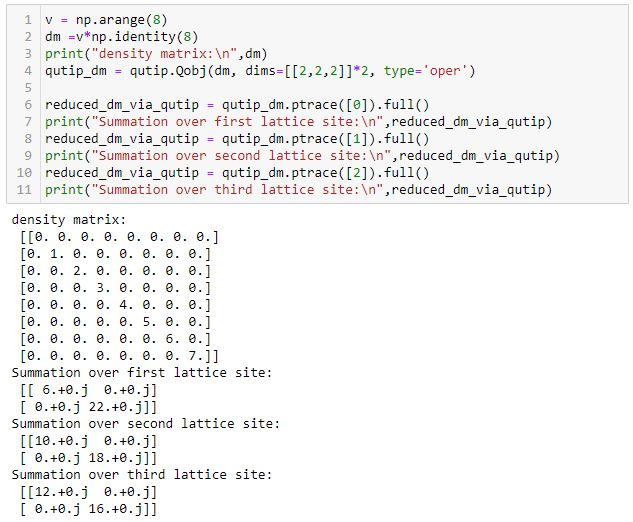
\includegraphics[width=0.7\linewidth]{figures/partialtrace_proof_of_concept}
\caption{Proof of concept for partial trace calculation similar to \protect\hyperlink{http://qutip.org/docs/3.1.0/guide/guide-tensor.html}{QuTiP-Guide/ptrace}.}
\label{fig:partialtrace_proof_of_concept}
\end{figure}

The algorithm of selecting the position vector of $n$ consecutive sites was implemented as follows: 
\begin{enumerate}
	\item Find the center spin rounded to next lowest integer.
	\item Determine left chain length $n_\text{left}$ as $n/2$ rounded to the next lowest integer.
	\item Determine right chain length $n_\text{right}$ as $n-n_\text{left}$.
	\item Select spins from left chain end to right chain end around center spin.
\end{enumerate}
This results in a behavior that picks left indices more favorably, but succeeds if equally spaced ends exist. Let the spins be numbered as $\{1, 2, 3, 4, 5\}$ for $N=5$, then  $n=3$ results in $\{2, 3, 4\}$, whereas $n=2$ results in $\{2, 3\}$.

These lattice sites serve then as an input to the partial trace function, such that the density matrix represents the measurement statistics of the center system.

\subsection{Machine learning models and error metrics}\label{sec:nn}

The decision for the machine learning framework \texttt{keras} was motivated by its flexibility and simplicity. \cite{chollet2015keras}

When setting up the machine learning model, one can already specify the first and last layer: The first (input) layer has to match the sample size of the incoming data, this can be already computed in advance. The length $len$ for block size $n$ is $2\cdot\left(2^n\times 2^n \right)$. The factor 2 comes from a preprocessing step, where the complex values are mapped to a second real picture, since the fitting procedure usually does not expect complex numbers. The last layer is a one node sigmoid, as the target output is the one-dimensional classification in $\left[0,1\right]$.

For small sample sizes, there exist various approaches to choose the right amount of layers and regularization methods \cite{Olson2018,Feng2019}, which cannot be generalized, as they heavily depend on feature size and target dimension. As a rule of thumb the approximation was used that each weight should be influenced by at least seven samples. Using this we get from 500 samples roughly 70 weights.
%todo: select amount of layers, nodes, dropout for regularization


The optimizer Adam was chosen, because it is computationally efficient,
has little memory requirements. \cite{Kingma2014}

For a two label classification problem, it is useful to use cross-entropy as a loss metric, as the penalty increases exponentially the further one deviates from the correct prediction.\cite{Goodfellow-et-al-2016}
\begin{figure}[h!]
\centering
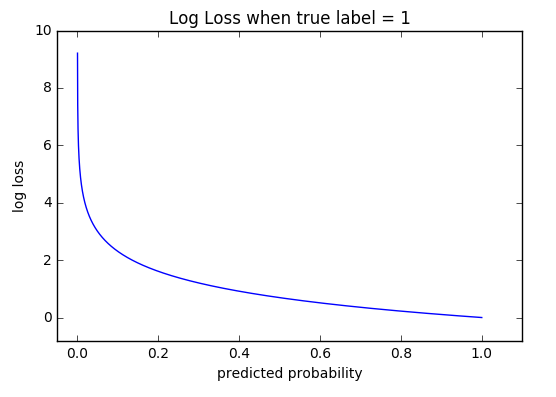
\includegraphics[width=\linewidth]{figures/cross_entropy}
\caption{Cross-Entropy Loss}
\label{fig:cross_entropy}
\end{figure}
The definition for a two class cross-entropy loss can be found in equation \ref{cross-loss}, where $y \in \{0,1\}$ is the true class and $\hat{y}\in\left[0,1\right]$ the predicted probability. This loss is also plotted in Figure \ref{fig:cross_entropy}.
\begin{equation}
L(\hat{y}, y)=-\left(y\log(\hat{y})+(1-y)\log(1-\hat{y})\right)\label{cross-loss}
\end{equation}

\subsection{Extraction of critical disorder strength $W_c$}\label{sec:wcextract}

To fit for the critical disorder strength $W_c$, two functions were compared. The logistic Fermi-Dirac like function:
\begin{align}
\text{L} \colon \;\mathbb {R} &\to \left[0,1\right]\\
\ W_{pred}&\mapsto \frac{1}{\exp\left(-\alpha \left(W_{pred}-W_c\right)\right)+1}
\end{align}
and the heaviside function:
\begin{align}
\text{H} \colon \;
\mathbb {R} &\to \{0,1\}\\
\ W_{pred}&\mapsto 
\begin{cases}
0:&W_{pred}<W_c\\1:&W_{pred}\geq W_c
\end{cases}
	\end{align}
The fully delocalized phase is defined as $0$ and fully localized as $1$. Whereas the heaviside function has an abrupt step and only maps to the extrema, the logistic function serves as a smoother option for a transition, depending on the parameter $alpha$. The motivation came also from an optimizers view: Differentiable functions are easier to fit for the computer.\cite{Kyurkchiev2015} Therefore, the logistic function was used to extract $W_c$ with the empiric decision of $\alpha=50$.

\subsection{Limitations for parameter range and resolution}\label{sec:param}

\begin{enumerate}
	\item System size $L$: Limited by computing time of eigenvalue solver. For the system size $L=12$, one calculation lasted approximately one minute.
	\item Block size $n$: 500 samples, $L=9$, $n=8$ required 4 GB of storage for the training set, exceeding the machines performance during model fitting. Therefore, $n=7$ was found to be sufficient for all system sizes.
	\item Sample size: 500 samples can be generated for $L=12$, $n_{max}=7$ in approximately 9 hours. This was found to be a sufficient sample size per system and block size.
	\item Disorder strength $W$ for the testing set: Since each point of a test set comes with a Hamiltonian with randomly drawn $h_i\in\left[-W,W\right]$, a decent amount of variance can be expected for the phase prediction. As we want to extract the phase change in general, and are not interested in the particular phase predictions of one specific Hamiltonian we choose to regularize the prediction by averaging over five predicted samples.
\end{enumerate}
%Training Set N=9 completed after 0.9669864177703857 seconds.
%Training Set N=10 completed after 5.634985685348511 seconds.
%Training Set N=11 completed after 25.606987714767456 seconds.
%Training Set N=12 completed after 139.2209861278534 seconds.



\section{Results}

\subsection{Generation of reduced density matrix training set}

The parameter range for the computation of the reduced density matrices can be found in Table \ref{tab:par_train}. The total computation time was 16.5 h, where 12.5 h where solely needed to compute the ground states of the $L=12$ system.

\begin{table}[h!]
	\centering
	\begin{tabular}{rl}
		\hline
		Parameter & Range or Set \\
		\hline
		\hline 
	\textbf{System size:} & $L \in \{9, 10, 11, 12\}$ \\ 
		\textbf{Block size:} & $n \in \{1, 2, 3, 4, 5, 6, 7\}$ \\ 
		\textbf{Repetitions:} & $r=500$\\
		\hline
	\end{tabular} 
	\caption{Parameter choice for training set generation}\label{tab:par_train}
\end{table}

In order to give some visual intuition, Figure \ref{fig:groundstate} shows realizations for different block sizes and phases.
\newpage\onecolumngrid
\begin{center}
	\begin{figure}[H]
		\centering	
		\begin{subfigure}[c]{0.45\textwidth}
			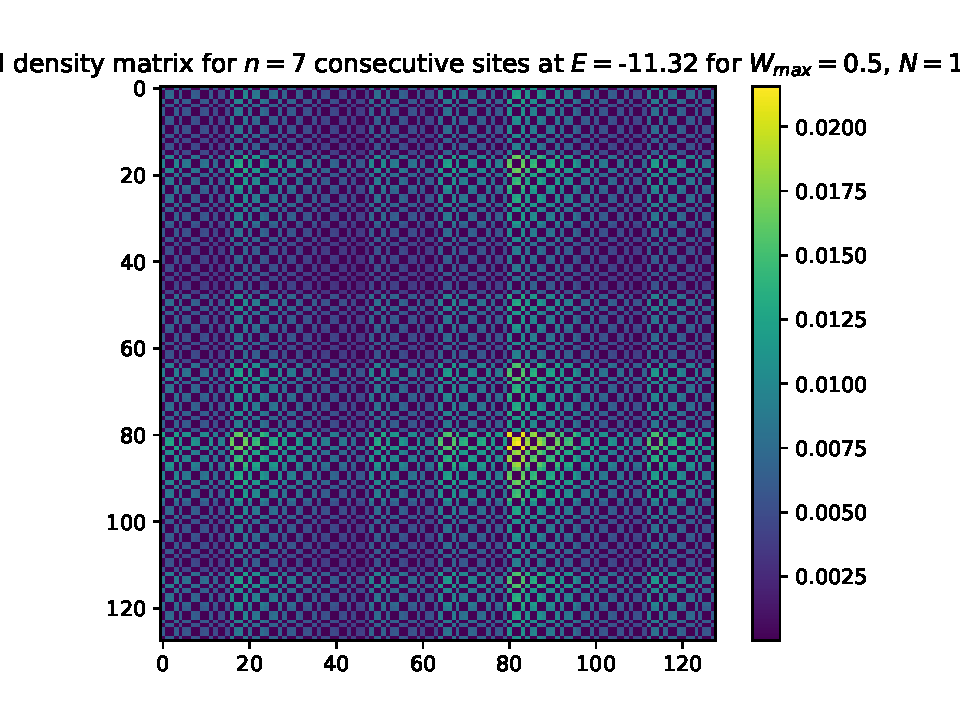
\includegraphics[width=\textwidth]{../results/groundstates/N12n7_trainingset_groundstate_Wmax0.5.pdf}
			\subcaption{extended phase, $n=7$.}
		\end{subfigure}
		\begin{subfigure}[c]{0.45\textwidth}
			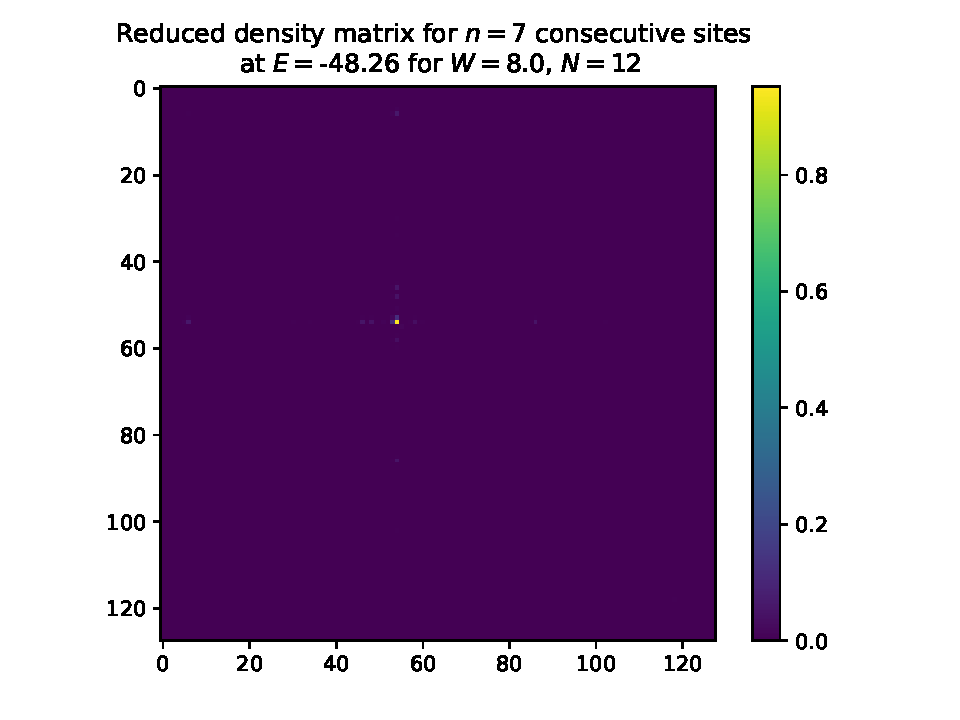
\includegraphics[width=\textwidth]{../results/groundstates/N12n7_trainingset_groundstate_Wmax8.0.pdf}
			\subcaption{localized phase, $n=7$.}
		\end{subfigure}
		\begin{subfigure}[c]{0.45\textwidth}
			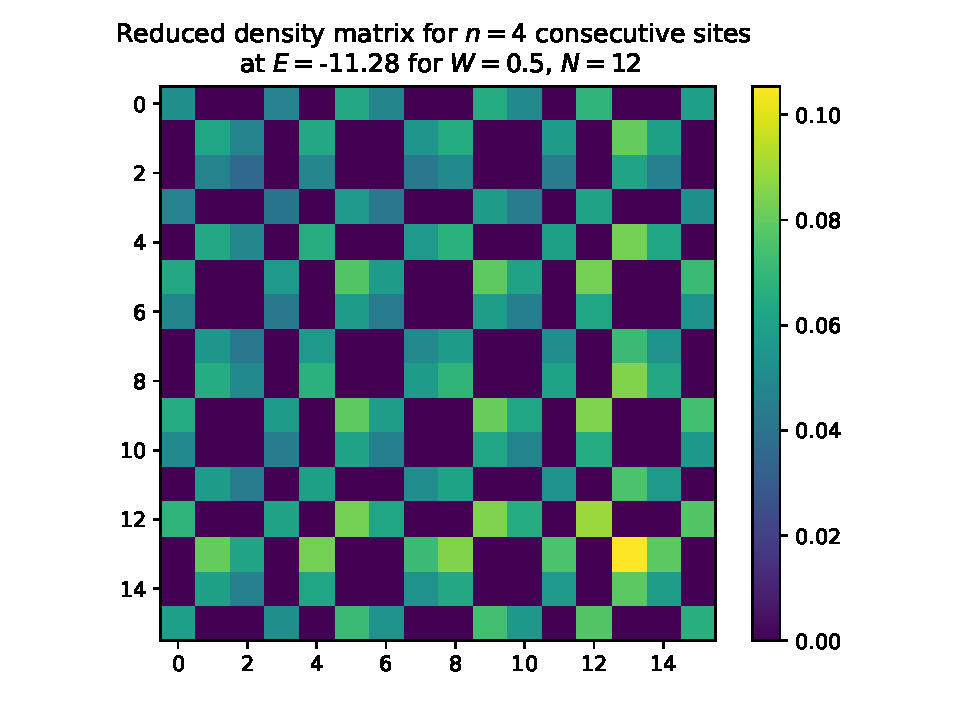
\includegraphics[width=\textwidth]{../results/groundstates/N12n4_trainingset_groundstate_Wmax0.5.pdf}
			\subcaption{extended phase, $n=4$.}
		\end{subfigure}
		\begin{subfigure}[c]{0.45\textwidth}
			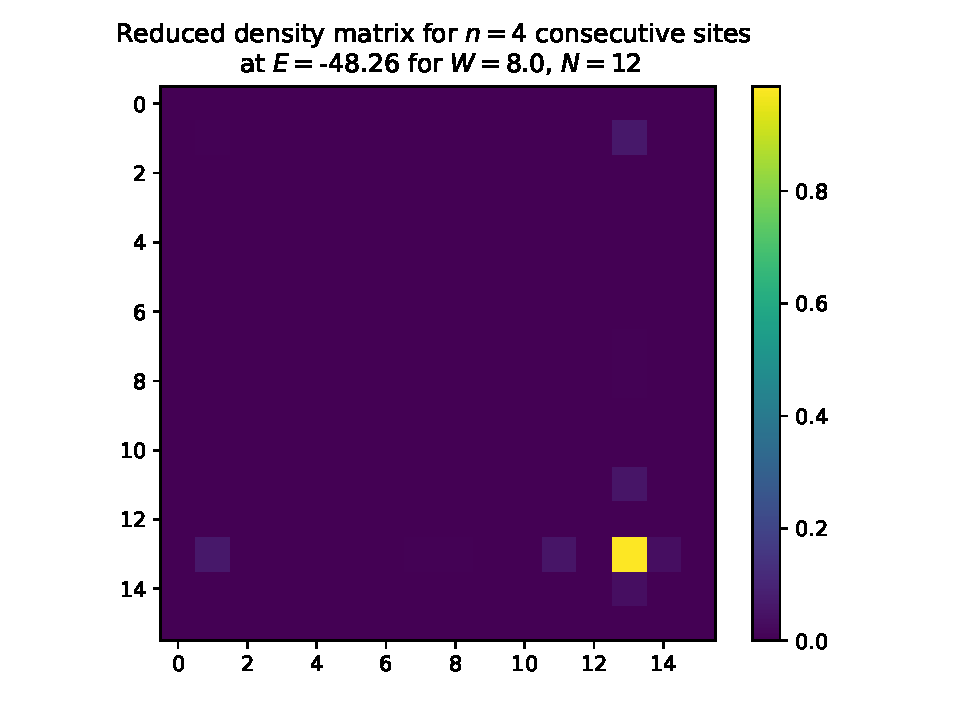
\includegraphics[width=\textwidth]{../results/groundstates/N12n4_trainingset_groundstate_Wmax8.0.pdf}
			\subcaption{localized phase, $n=4$.}
		\end{subfigure}
		\begin{subfigure}[c]{0.45\textwidth}
			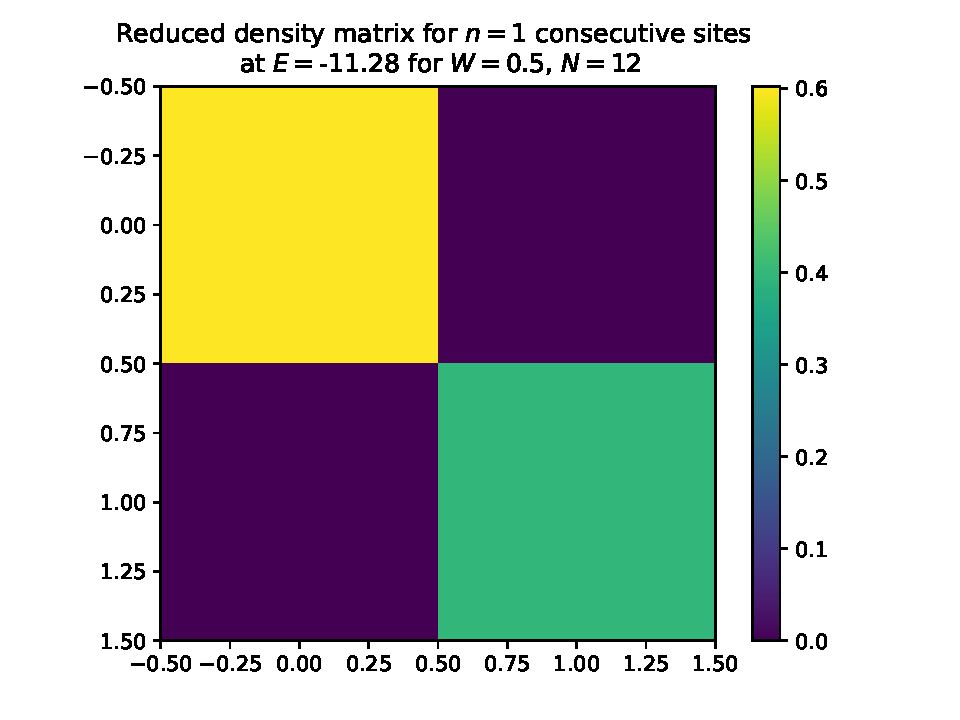
\includegraphics[width=\textwidth]{../results/groundstates/N12n1_trainingset_groundstate_Wmax0.5.pdf}
			\subcaption{extended phase, $n=1$.}
		\end{subfigure}
		\begin{subfigure}[c]{0.45\textwidth}
			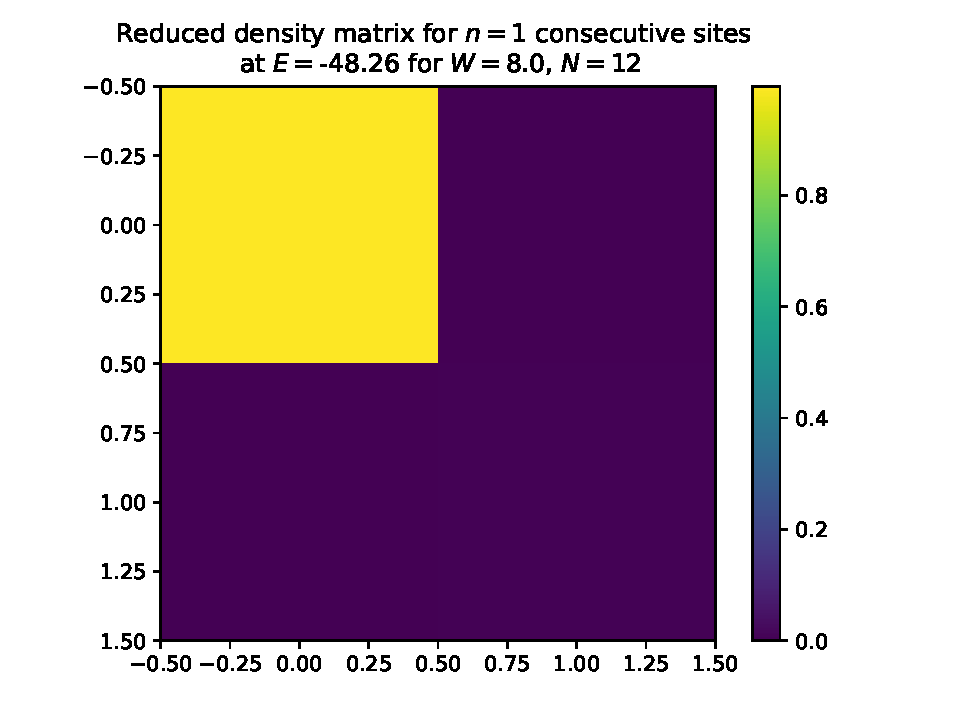
\includegraphics[width=\textwidth]{../results/groundstates/N12n1_trainingset_groundstate_Wmax8.0.pdf}
			\subcaption{localized phase, $n=1$.}
		\end{subfigure}
		\caption{Real part of the density matrix of an ergodic and localized phases for block sizes $n=\{4, 5\}$ and system size $L=12$.}
		\label{fig:groundstate}
	\end{figure}
\end{center}
\twocolumngrid\newpage
The visual inspection indicates that the density matrix of the localized phase has a sharp maximum at the preferred state that is forced by the random disorder strength. The extended phase shows a checkerboard pattern structure, which reflects that some configurations are more preferred than others. These energetically expensive states are related to neighboring unaligned spins. Another observation is that the density matrix reductions of the full ground state conserved these properties for $n>2$, when comparing $n=7$ to $n=\{6,5,4,3,2\}$. The similarity between the two phases gets smaller the smaller the block size $n$. For $n=1$, one could argue that the density matrices are very similar, as they only deviate for half the matrix elements.

%todo: Measure of variation in the test set??

%\begin{figure}
%	\begin{subfigure}[c]{0.2\textwidth}
%			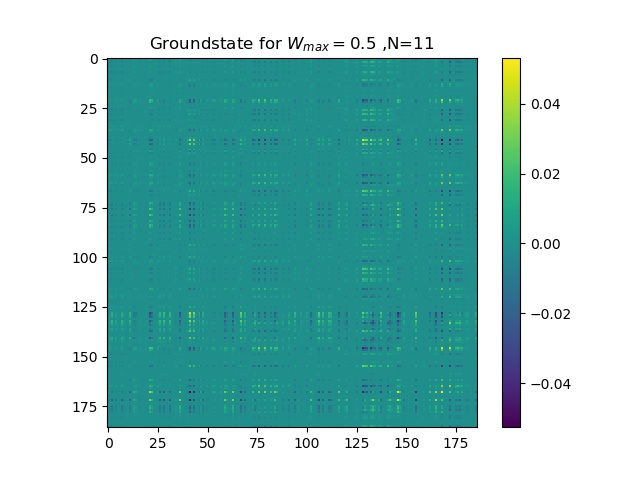
\includegraphics[width=\textwidth]{../results/N11_trainingset_groundstate_Wmax0.5.jpg}
%		\subcaption{}
%	\end{subfigure}
%	\begin{subfigure}[c]{0.2\textwidth}
%		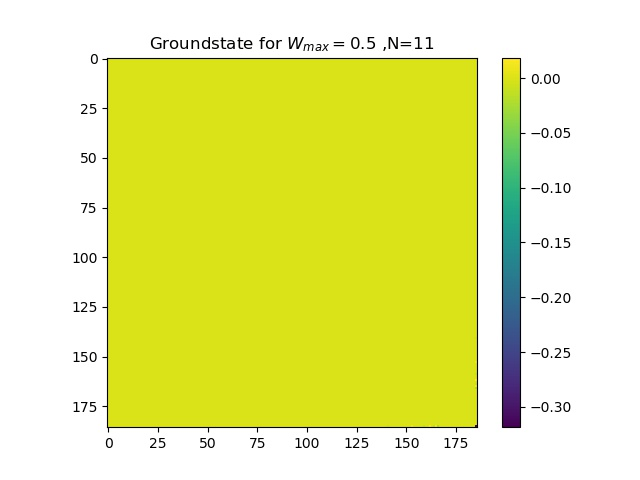
\includegraphics[width=\textwidth]{../results/N11_trainingset_groundstate_Wmax8.0.jpg}
%		\subcaption{}
%	\end{subfigure}
%	\caption{Zwei Bilder mit Subfigure nebeneinander}
%\end{figure}

\subsection{Model training}\label{sec:loss_acc}

Before we can predict the phase of a newly generated test set, we have to train the neural network with our available training data. For each system and block size a separate model was trained, as a different system size might influence the physical behavior due to open boundary conditions.

The neural networks are generated as a sequential keras model with the following configuration, as discussed in section \ref{sec:nn}: 

\begin{lstlisting}[language=Python]
model = models.Sequential()
model.add(layers.Flatten(input_shape=(np.shape(self.X_train)[1], np.shape(self.X_train)[1], 2)))
model.add(layers.Dense(64, activation='relu', bias_regularizer='l2'))
model.add(layers.Dense(64, activation='relu', bias_regularizer='l2'))
model.add(layers.Dense(1, activation='sigmoid'))
model.compile(optimizer='adam', loss='binary_crossentropy', metrics=['accuracy'])
\end{lstlisting}

Two strategies are employed to prevent over-fitting:
\begin{enumerate}
	\item $30$ \% of the training set was used for validation. To avoid a biased split, we relied on \texttt{sklearn}'s method \texttt{train\_test\_split} that samples randomly from the training set.
	\item A bias regularizer was introduced to move the output functions closer to the origin. Even though some further regularization might still be possible, a kernel regularizer did not prove to be useful and impacted the resulting scores heavily.
\end{enumerate}

The model training was executed by using a batch size of 70 and 200 epochs, where the batch size was limited by the CPU performance and no significant loss or accuracy improvements where noted after 120 epochs.

An example of the accuracy and loss dependency on the number of epochs for system size $L=10$, and block sizes $n=\{1, 7\}$ is presented below in Figure \label{fig:val_acc}.%todo: more training epochs

\onecolumngrid
\begin{center}%todo: loss, accuracy heatmap plot
	\begin{figure}[H]
		\centering	
		\begin{subfigure}[c]{0.45\textwidth}
			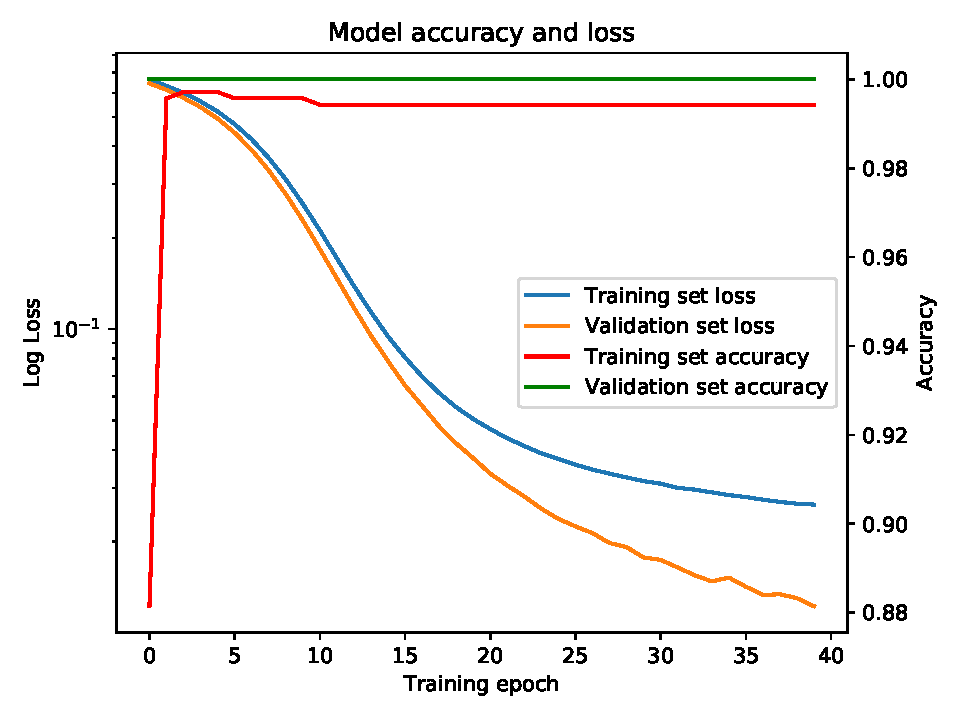
\includegraphics[width=\textwidth]{../results/accuracy_loss_epochs/N10n1_accuracy_loss_epochs.pdf}
			\subcaption{$n=1$}
		\end{subfigure}
		\begin{subfigure}[c]{0.45\textwidth}
			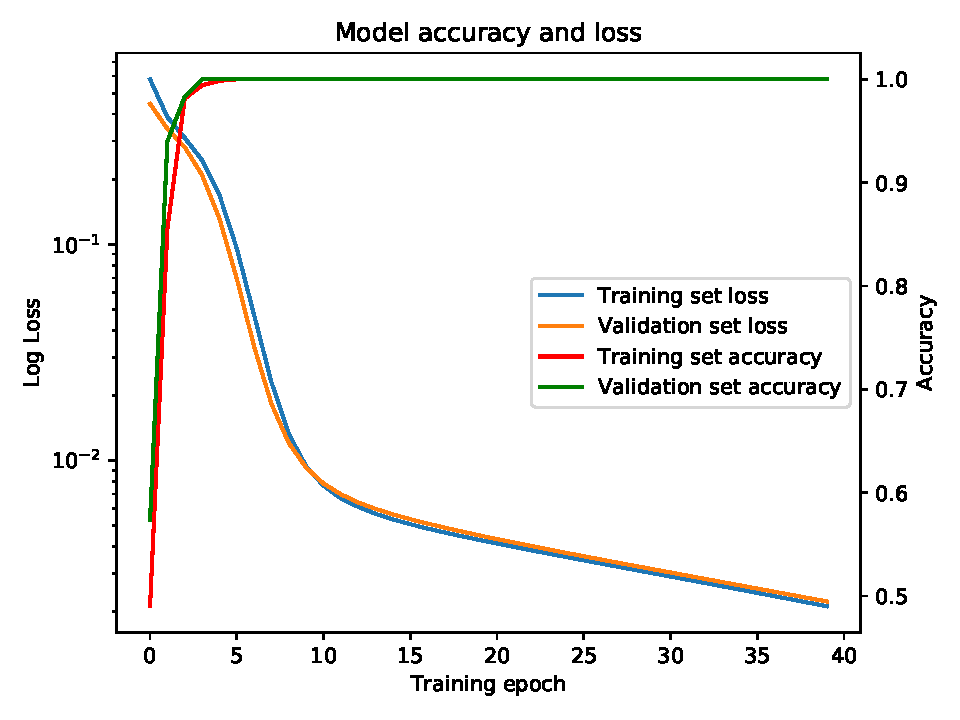
\includegraphics[width=\textwidth]{../results/accuracy_loss_epochs/N10n7_accuracy_loss_epochs.pdf}
			\subcaption{$n=7$}
		\end{subfigure}
		\caption{Loss and accuracy on training and validation set for system size $L=10$.}
		\label{fig:val_acc}
	\end{figure}
\end{center}
\twocolumngrid

The overall losses for $n>1$ where always found to be $\approx 0.01$ with accuracies of $1.0$, whereas the models at $n=1$ showed larger losses of  $\approx 0.1$ and mostly acceptable accuracies near $1$.

Figure \ref{fig:val_acc} illustrates that not only the scores for small block sizes were lower, but also the convergence rates. In conclusion, the scores show that the learning of the phases was prone to severe over-fitting and resulted in acceptable scores for the next step of prediction, where $n=1$ can be expected to have a worse performance during the prediction. This behavior was expected, when we notized the similarity for $n=1$ block size samples in the training set.

\subsection{Analysis of critical disorder strength}
\subsubsection{Dependency on block size}
First, the testing set was generated. Following the parameter discussion in section \ref{sec:param}, we generate five samples for each $W\in\left[0,4\right]$, with step $\Delta W=0.05$, resulting in 400 samples per system and block size. Afterwards, the predictions were fitted with a logistic function to obtain $W_c$ as described in section \ref{sec:wcextract}.
Five predicted phases are averaged at each point and plotted to a heat map. The fitted $W_c$ is plotted along in Figure \ref{fig:wcextractn}.

\onecolumngrid
\begin{center}%todo: annotate colorbar
	\begin{figure}[H]
		\centering	
		\begin{subfigure}[c]{0.45\textwidth}
			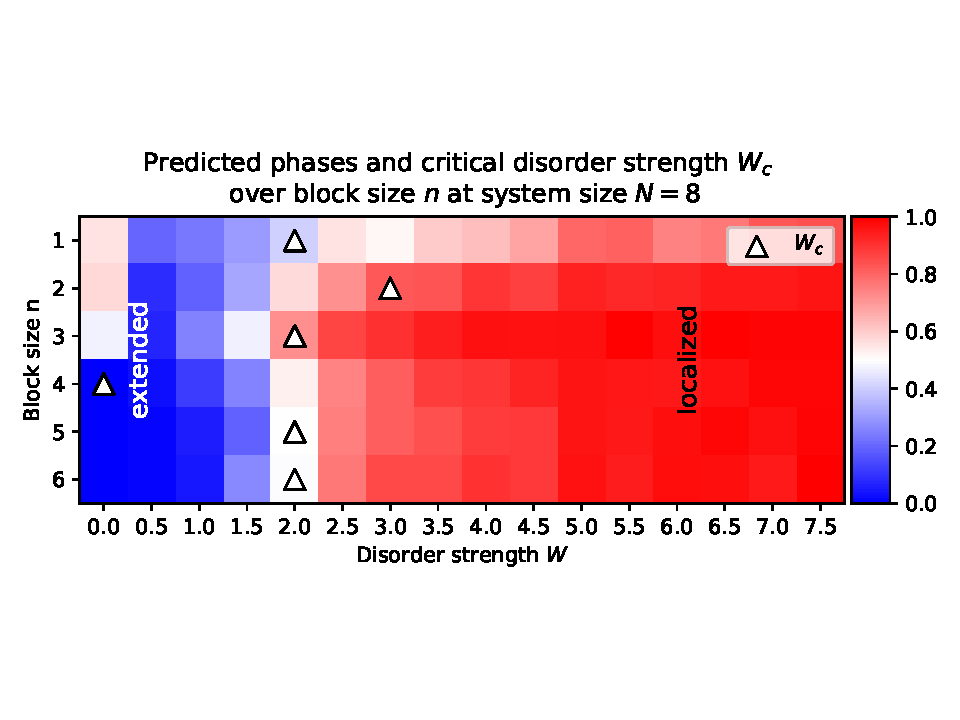
\includegraphics[width=\textwidth]{../results/Wc/N8_Wc_n_dependency.pdf}
			\subcaption{$L=8$}
		\end{subfigure}
		\begin{subfigure}[c]{0.45\textwidth}
			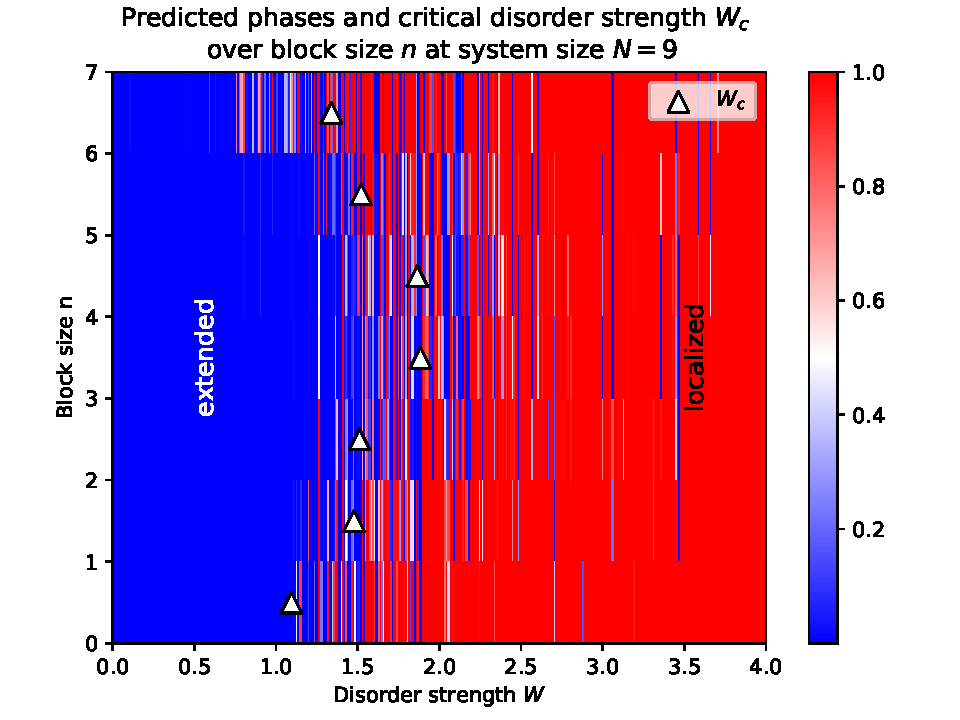
\includegraphics[width=\textwidth]{../results/Wc/N9_Wc_n_dependency.pdf}
			\subcaption{$L=9$}
		\end{subfigure}
		\begin{subfigure}[c]{0.45\textwidth}
			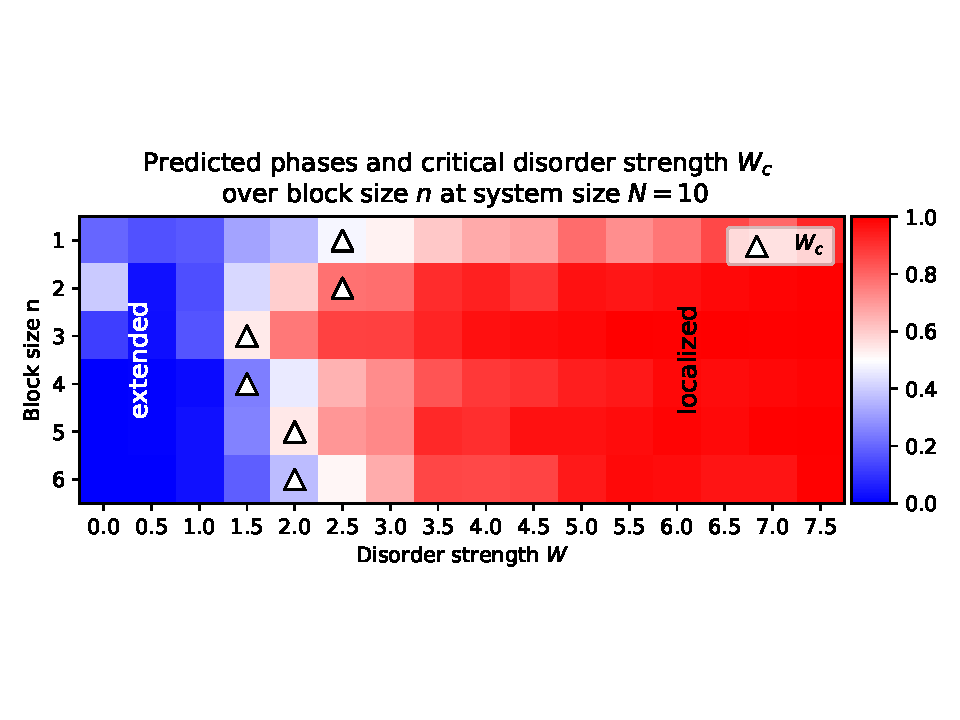
\includegraphics[width=\textwidth]{../results/Wc/N10_Wc_n_dependency.pdf}
			\subcaption{$L=10$}
		\end{subfigure}
		\begin{subfigure}[c]{0.45\textwidth}
			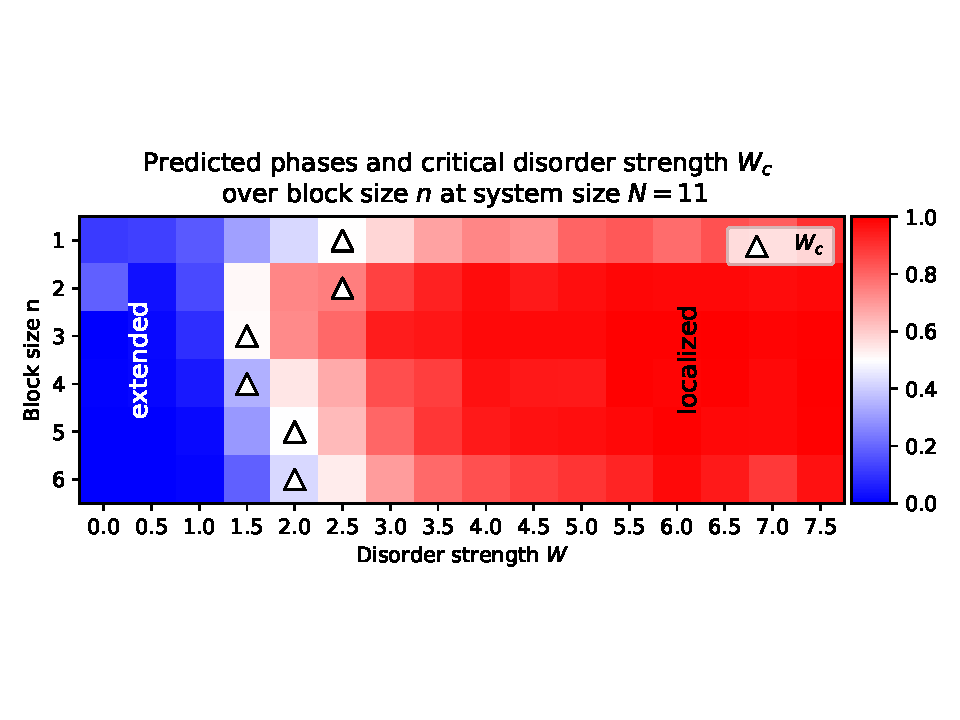
\includegraphics[width=\textwidth]{../results/Wc/N11_Wc_n_dependency.pdf}
			\subcaption{$L=11$}
		\end{subfigure}
		\begin{subfigure}[c]{0.45\textwidth}
			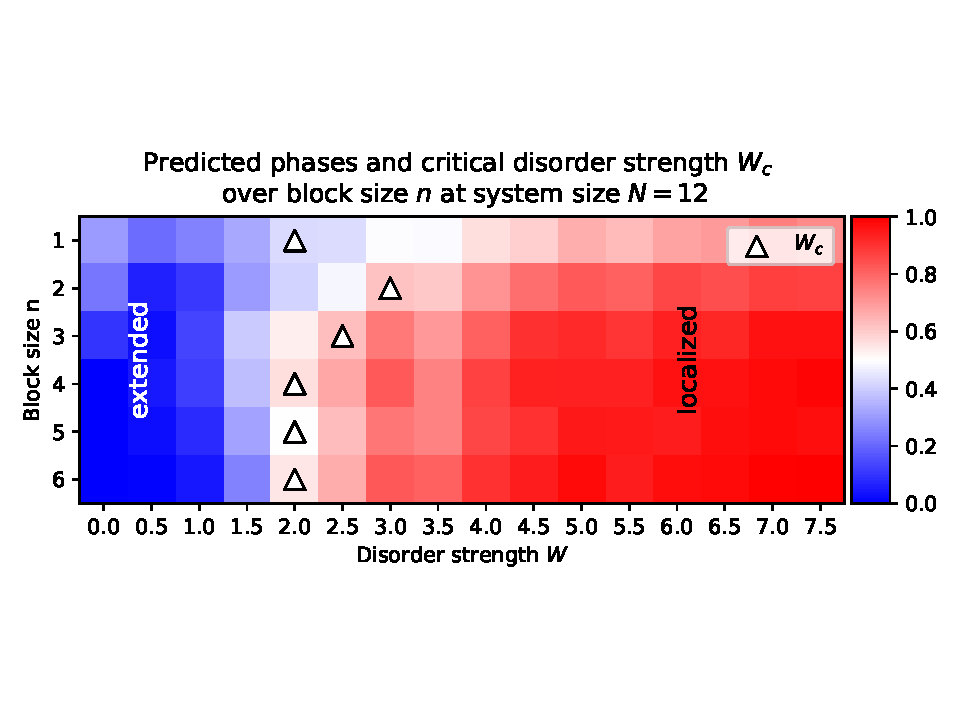
\includegraphics[width=\textwidth]{../results/Wc/N12_Wc_n_dependency.pdf}
			\subcaption{$L=12$}
		\end{subfigure}
		\caption{Dependency of the phase transition on block size $n$ for different system sizes.}
		\label{fig:wcextractn}
	\end{figure}
\end{center}
\twocolumngrid

In conclusion, the predicted critical disorder strength $W_c$ decayed, when models with larger block sizes $n$ were used for prediction. The low $W_c$ values for $n=\{1,2\}$ might just as well be attributed to the poor loss and accuracy values shown in section \ref{sec:loss_acc}. An explanation for this decay might be that a bigger block size can more accurately reflect the level of disorder forced on the system. For smaller block sizes, for some spins the information is lost whether the configuration was the result of interacting lattice sites or the random disorder strength.

\subsubsection{Dependeny on system size}

something something%todo: write


\onecolumngrid
\begin{center}
	\begin{figure}[H]
		\centering	
		\begin{subfigure}[c]{0.4\textwidth}
			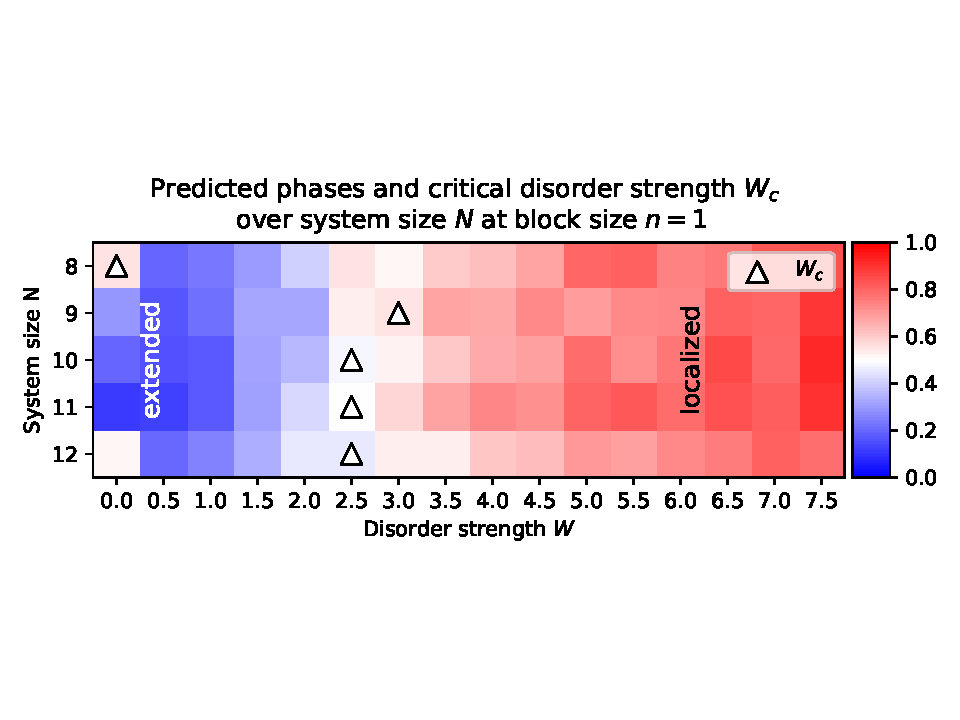
\includegraphics[width=\textwidth]{../results/Wc/n1_Wc_N_dependency.pdf}
			\subcaption{$n=1$}
		\end{subfigure}
		\begin{subfigure}[c]{0.4\textwidth}
			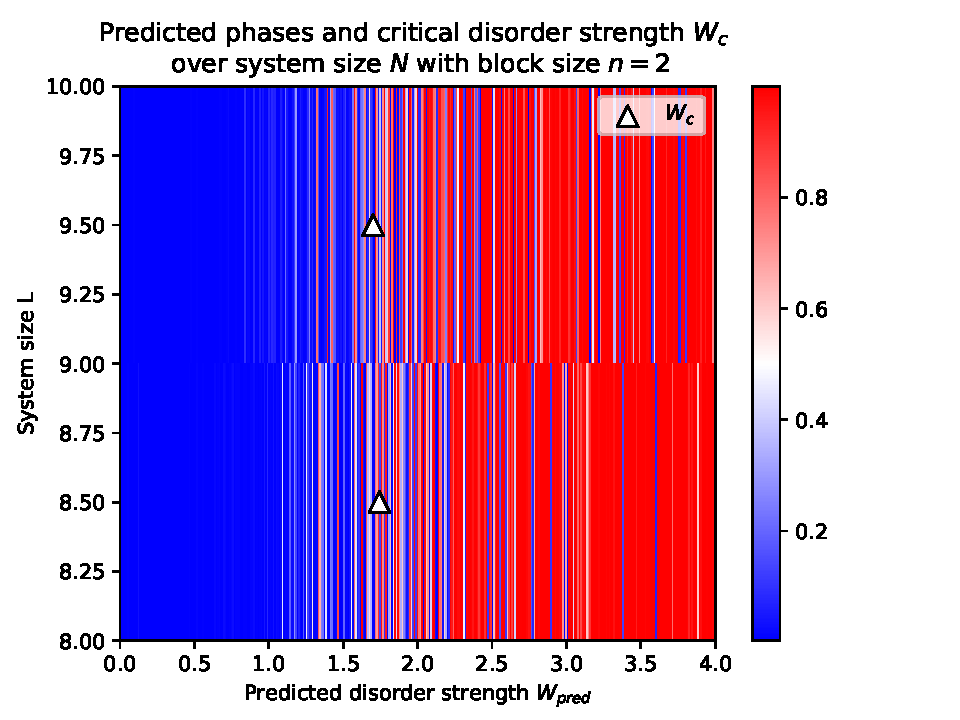
\includegraphics[width=\textwidth]{../results/Wc/n2_Wc_N_dependency.pdf}
			\subcaption{$n=2$}
		\end{subfigure}
		\begin{subfigure}[c]{0.4\textwidth}
			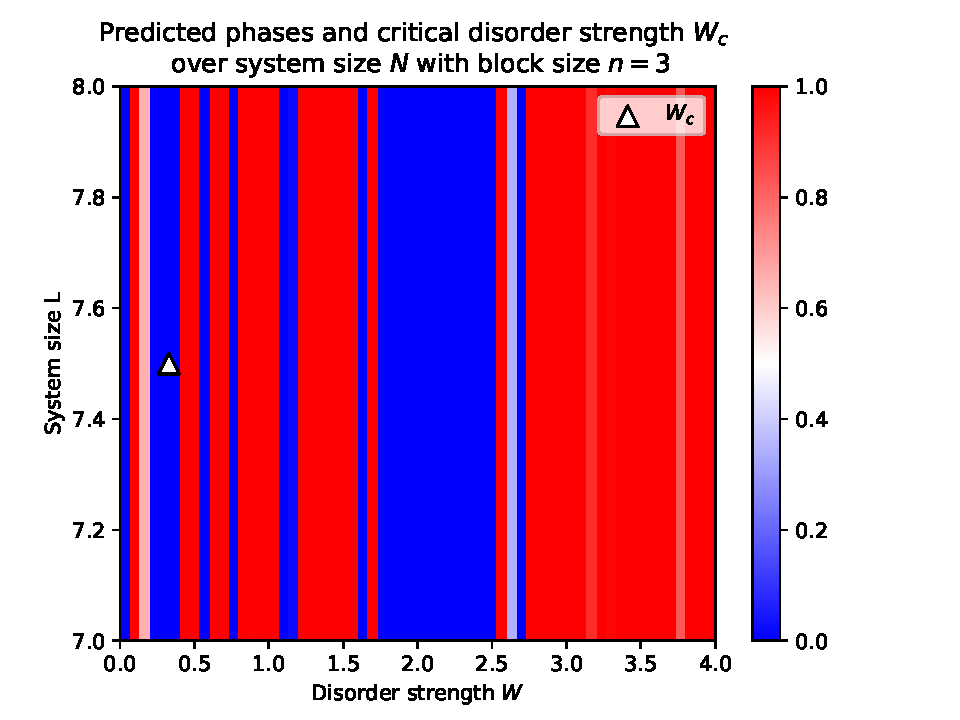
\includegraphics[width=\textwidth]{../results/Wc/n3_Wc_N_dependency.pdf}
			\subcaption{$n=3$}
		\end{subfigure}
		\begin{subfigure}[c]{0.4\textwidth}
			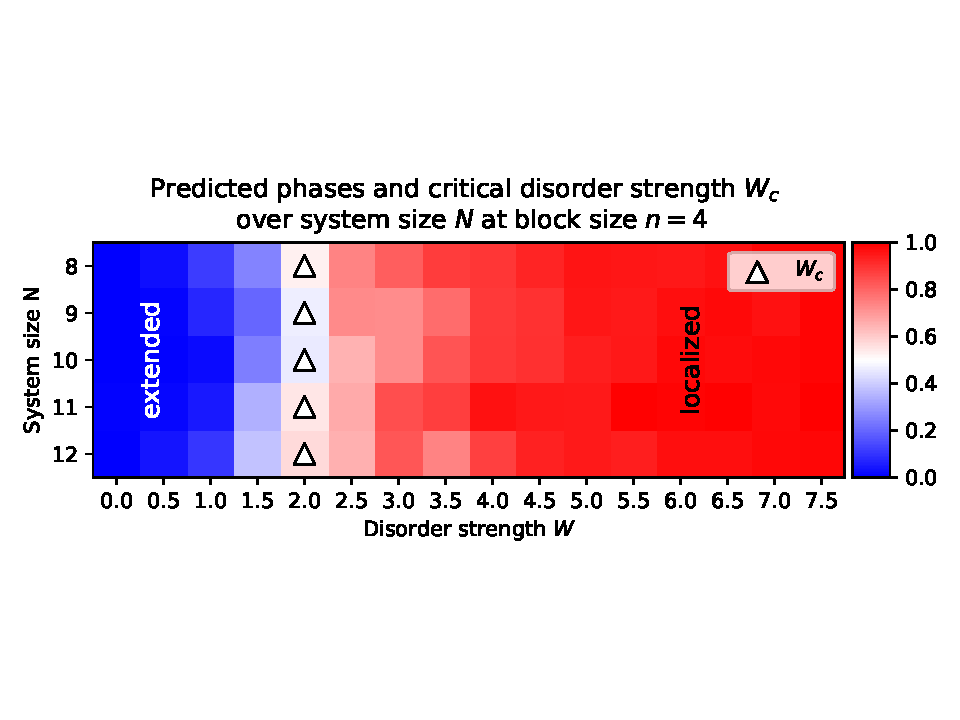
\includegraphics[width=\textwidth]{../results/Wc/n4_Wc_N_dependency.pdf}
			\subcaption{$n=4$}
		\end{subfigure}
		\begin{subfigure}[c]{0.4\textwidth}
			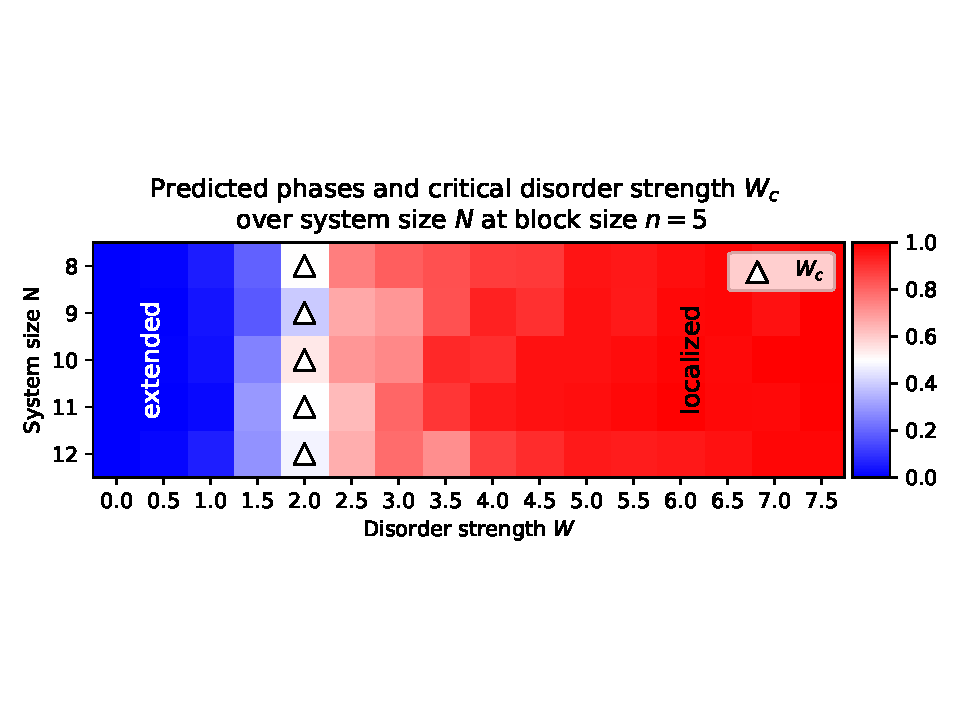
\includegraphics[width=\textwidth]{../results/Wc/n5_Wc_N_dependency.pdf}
			\subcaption{$n=5$}
		\end{subfigure}
		\begin{subfigure}[c]{0.4\textwidth}
			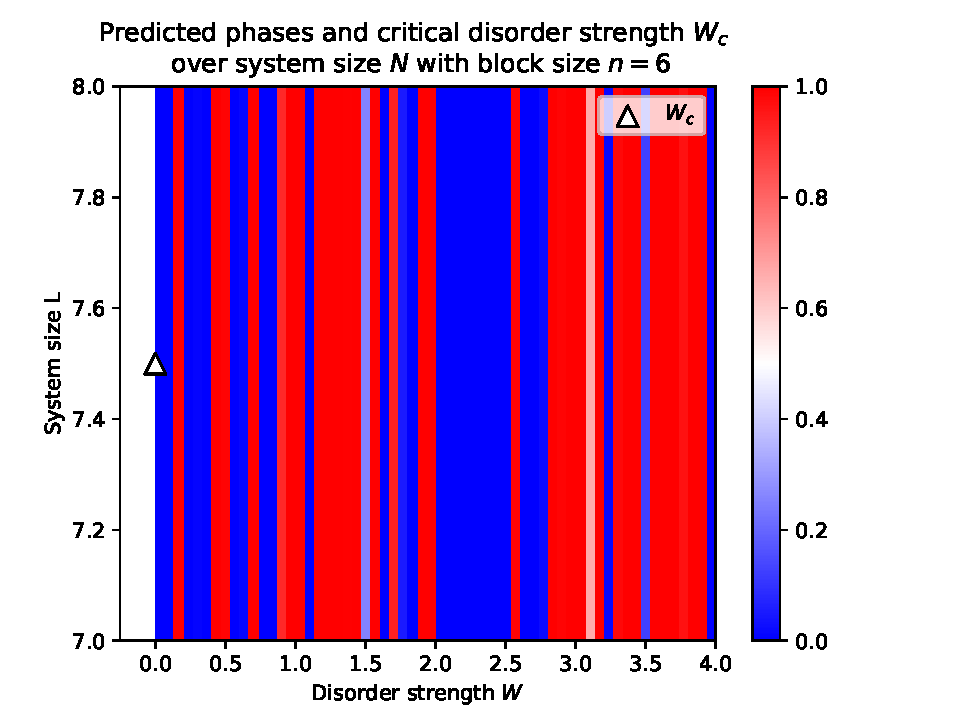
\includegraphics[width=\textwidth]{../results/Wc/n6_Wc_N_dependency.pdf}
			\subcaption{$n=6$}
		\end{subfigure}
		\begin{subfigure}[c]{0.4\textwidth}
			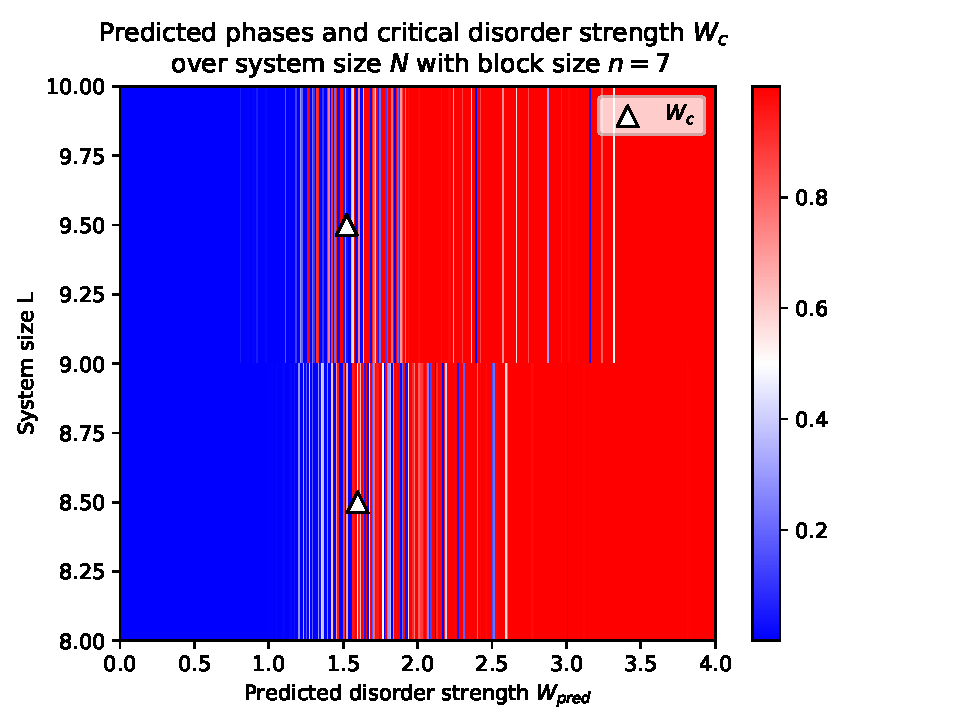
\includegraphics[width=\textwidth]{../results/Wc/n7_Wc_N_dependency.pdf}
			\subcaption{$n=7$}
		\end{subfigure}
		\caption{Dependency of the phase transition over system sizes $L$ for different block sizes $n$.}
		\label{fig:wcextract}
	\end{figure}
\end{center}
\twocolumngrid%todo: compare with introduction


%todo: Plot N dependency
The plots are indicating that a bigger system size requires a larger disorder strength to perform the phase transition.


\section{Conclusion}%todo: Action title

$W_c$ depends on n, L (yes/no).

$W_c$ prediction coincides with the expectation (yes/no)

$W_c$ is dependent on these and that effects => scaling analysis? (yes/no)

\lipsum[2]%todo: write

\bibliography{zotero}
%\bibliography{bibsamp}% Produces the bibliography via BibTeX.

\newpage
\appendix


\begin{widetext}
\section{Code listing} \label{app:codes}
The code consists essentially of five different files, which are callable through a main function, but can also be run separately. Every file serves a number of different purposes as listed below.

\begin{enumerate}
	\item \textbf{generate\_training\_set.py}: Here, the training set is generated and some example plots of ground states are saved to the results folder. The training sets are saved in the \texttt{training\_sets} folder, where they are numbered with their system and block size.
	\item \textbf{ed.py}: The training set is generated by using the functions from the tutorial. A new function was added that generates the Hamiltonian using the random local disorder strength.
	\item \textbf{model\_save\_train.py}: First, models are generated that automatically match the input data of different block sizes $n$, afterwards, they are trained with a certain amount of epochs and batch sizes. The history of the validation and accuracy is plotted individually into the results folder.
	\item \textbf{generate\_test\_set.py}: A set of reduced density matrices for ground states in the intermediate regime is generated.
	%todo: plot state near W=1
	\item \textbf{load\_model\_get\_wc.py}: The models for each system and block size make phase predictions to the respective test sets, extract $W_c$ and plot everything together as a heat map.
\end{enumerate}

\subsection{Training set generation}
\lstinputlisting[language=Python]{../generate_training_set.py}

\subsection{Model Training}
\lstinputlisting[language=Python]{../model_save_train.py}

\subsection{Test set generation}
\lstinputlisting[language=Python]{../generate_test_set.py}

\subsection{Prediction and evaluation of $W_c$}
\lstinputlisting[language=Python]{../load_model_get_wc.py}

\subsection{Exact diagonalization}
\lstinputlisting[language=Python]{../ed.py}
%\begin{lstlisting}[language=Python]
%%\include{file}
%\include{}
%\end{lstlisting}
\end{widetext}



\end{document}
